\section{Exlurs: Lamé'schen Kurve}

Um einen Kreis schrittweise in ein Quadrat zu verwandeln, nutzt man die sogenannte Superellipse (auch Lamesche Kurve genannt) oder mathematisch gesprochen den Übergang zur $p$ Norm (auch Manhattan- oder Maximum-Metrik genannt).

Die modifizierte Formel lautet:
\begin{equation}
    R_{p}(x,y) = 
    \left(|x|^{p}+|y|^{p}\right)^{\frac{1}{p}}
\end{equation}

Wenn man den Exponenten $p$ erhöht, flachen die Rundungen des Kreises immer weiter ab, und die Kurve nähert sich einem Quadrat an.

Die mathematische Entwicklung
\begin{itemize}
    \item  $p = 2$ (Startwert): Das ist der klassische euklidische Abstand. Die Gleichung $R(x,y) = 1$ beschreibt einen Kreis.
    \item  $p = 4, 8, 16 \dots$: Je größer $p$ wird, desto flacher werden die Kurvensegmente und desto schärfer werden die Ecken. Es entsteht ein \glqq Superkreis\grqq (Squircle).
    \item  $p \to \infty$ (Grenzwert): Im Unendlichen wird die Formel zur Maximum-Metrik: $R(x, y) = \max(\vert{}x\vert{}, \vert{}y\vert{})$. Das Ergebnis ist ein Quadrat.
\end{itemize} 

Hier ist die visuelle Transformation für verschiedene Werte von $p$:

\begin{figure}[htbp]
    \centering
    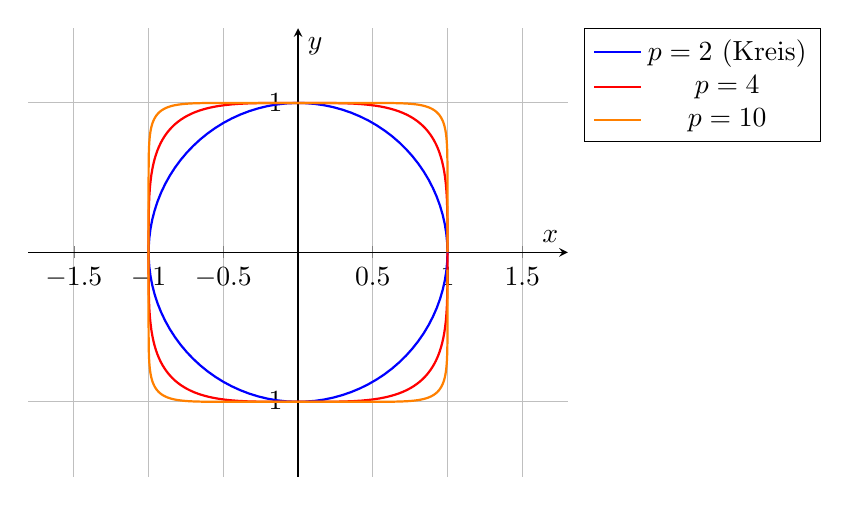
\begin{tikzpicture}
        \begin{axis}[
            axis lines=middle,
            xmin=-1.5, xmax=1.5,
            ymin=-1.5, ymax=1.5,
            xlabel={$x$}, ylabel={$y$},
            axis equal, % Verhindert Verzerrungen (wichtig für Kreise/Quadrate)
            grid=major,
            legend pos=outer north east
        ]
            
            % 1. Klassischer Kreis (p = 2) -> Exponent 2/2 = 1
            \addplot[
                blue, thick, samples=100, domain=0:360
            ] ({cos(x)}, {sin(x)});
            \addlegendentry{$p = 2$ (Kreis)}
            
            % 2. Lamé-Kurve (p = 4) -> Exponent 2/4 = 0.5
            % Da pgfmath Probleme mit negativen Basen hat, nutzen wir abs()
            \addplot[
                red, thick, samples=150, domain=0:360
            ] (
                {sign(cos(x)) * abs(cos(x))^(2/4)}, 
                {sign(sin(x)) * abs(sin(x))^(2/4)}
            );
            \addlegendentry{$p = 4$}
            
            % 3. Lamé-Kurve (p = 10) -> Nähert sich stark dem Quadrat an
            \addplot[
                orange, thick, samples=200, domain=0:360
            ] (
                {sign(cos(x)) * abs(cos(x))^(2/10)}, 
                {sign(sin(x)) * abs(sin(x))^(2/10)}
            );
            \addlegendentry{$p = 10$}
            
        \end{axis}
    \end{tikzpicture}
    \caption{Visualisierung der Lamé'schen Kurve für verschiedene Exponenten $p$.}
    \label{fig:lame_kurve}
\end{figure}


Die modifizierte Formel für die Annäherung an ein Quadrat lautet:
\begin{equation}
    R_p(x, y) = \sqrt[p]{|x|^p + |y|^p} \quad \text{mit } p \ge 2
\end{equation}
Für $p \to \infty$ konvergiert die Formel gegen die Maximum-Norm $R_\infty(x, y) = \max(|x|, |y|)$, welche gegen ein Quadrat konvergiert.

\newpage
